\section{Additional tables}
\begin{table}[h]
\caption{\textbf{Full calibration table (T0)}, $\tau\in\{0,0.1\}$, $K=200$, $n\in\{100,500\}$, 1000 replicates per cell; columns as Table~\ref{tab:C}.}
\label{tab:Cfull}
\centering\scriptsize
\resizebox{\linewidth}{!}{\input{../tables/table_c_calibration.tex}}
\end{table}
\begin{table}[h]
\caption{\textbf{Bootstrap optimism correction (M3) with the other methods (T0)}, $n=200$, $K=200$, 300 replicates per cell.}
\centering\scriptsize
\resizebox{\linewidth}{!}{\input{../tables/table_c_m3.tex}}
\end{table}
\begin{table}[h]
\caption{\textbf{Claim ``A beats B'' from reported scores (T0).} False-winner and detection rates (\%, Wilson 95\%).}
\label{tab:E}
\centering\scriptsize
\resizebox{\linewidth}{!}{\input{../tables/table_e_ab.tex}}
\end{table}
\begin{table}[h]
\caption{\textbf{Compute actually used.} Wall seconds per job on 2-vCPU containers of a shared host; the total is a sum of job times, not elapsed time. The scoring job's 81{,}172 s is first-to-last cached file of 8 parallel jobs; its tokens were not logged. The totals are job accounting: the separate leakage job (\texttt{t0leak}, 16 cells, 16{,}000 replicates) repeats cells that are also in the main grid, so the distinct synthetic grid is 216 cells and 203{,}400 replicates.}
\label{tab:F}
\centering\scriptsize
\input{../tables/table_f_compute.tex}
\end{table}
\begin{table}[h]
\caption{\textbf{Calibration on the real matrix (T1), $K=300$, $n\in\{100,500\}$}; columns as Table~\ref{tab:G}.  Uncertainty is $\pm1.96$ block SE; replicates share one pool (Limitation iv).}
\label{tab:Gfull}
\centering\scriptsize
\resizebox{\linewidth}{!}{\input{../tables/table_g_t1_calibration.tex}}
\end{table}
\begin{table}[h]
\caption{\textbf{False-winner and detection rates (\%, $\pm1.96$ block SE) for ``A beats B'' on the real matrix (T1), $n=100$.} ``point'': estimate of A exceeds that of B; ``lower bd'': A's lower bound exceeds B's estimate. Tuned-versus-baseline decisions are omitted: the baseline is almost always truly worse, so the false-claim rate is not identifiable.}
\label{tab:Hdec}
\centering\scriptsize
\resizebox{\linewidth}{!}{\input{../tables/table_h_t1_decisions.tex}}
\end{table}
\begin{figure}[h]
\centering
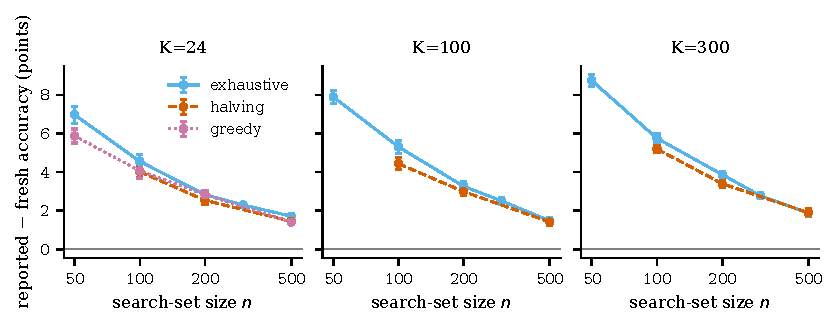
\includegraphics[width=\linewidth]{fig_b_t1.pdf}
\caption{\textbf{Search procedure (T1).} Optimism by exhaustive, successive-halving and greedy search (greedy only at $K=24$); panels $K=24,100,300$; $\pm1.96$ block SE.}
\label{fig:B1}
\end{figure}
\begin{figure}[h]
\centering
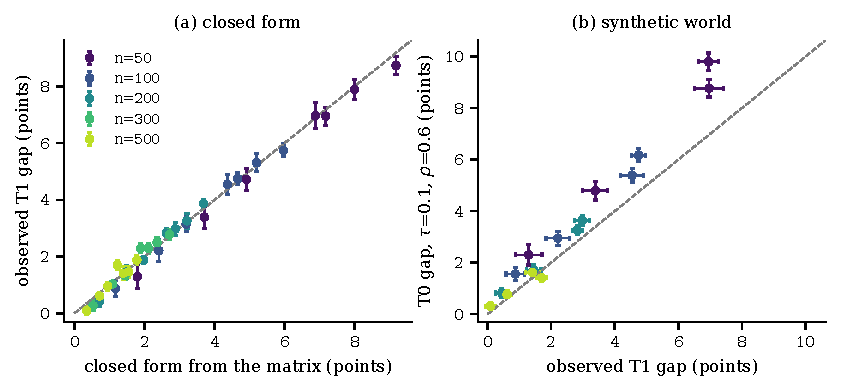
\includegraphics[width=\linewidth]{fig_t1_check.pdf}
\caption{\textbf{Checks of the extreme-value form and of the synthetic world against the real matrix (T1).} (a) Observed gap against the closed form fed with the matrix's $(\sigma,r,\tau)$, all 35 exhaustive cells. (b) Observed T1 gap against the T0 cells with the same $(n,K)$ at $\tau=0.1$, $\rho=0.6$ and baseline accuracy 0.3 (T0 is not calibrated to the matrix); dashed: $y=x$.}
\label{fig:T1check}
\end{figure}
\begin{figure}[h]
\centering
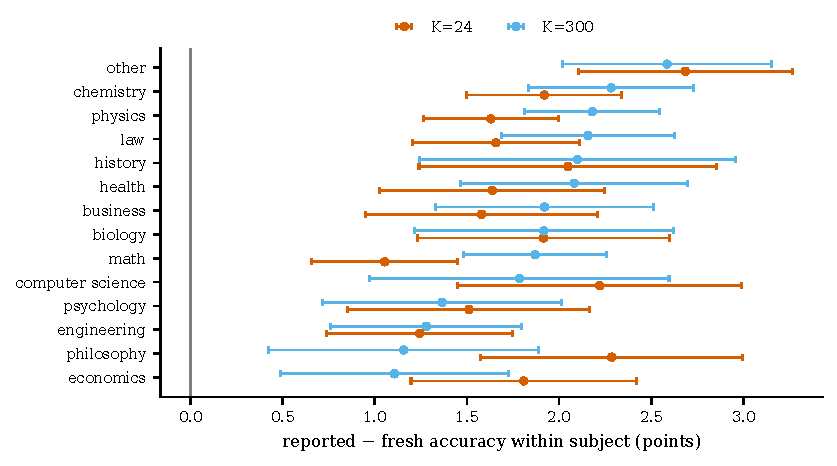
\includegraphics[width=\linewidth]{fig_t1_subjects.pdf}
\caption{\textbf{Gap by MMLU-Pro subject (T1)}, $n=500$, $K=24$ and $300$. A subject holds 16--63 of the 500 search items and replicates share items, so the bars understate uncertainty; the figure shows that optimism is present in every subject, not differences between subjects.}
\label{fig:T1subj}
\end{figure}
